%%=====================================================================
%% RESULTADOS: simulação por partes, ganhos, ensaio, placas
%% Slides com \ilustrativo trazem dados provisórios: substituir.
%%=====================================================================
\begin{frame}{Estimação em partes}
  \centering
  \tikzfig{1}{0.72}{smo_hibrido}
  \fonte[Adaptado de Utkin (1992); Abo Kaf et al.\ (2024)]
\end{frame}

\begin{frame}{Inversor simulado}
  \centering
  \tikzfig{1}{0.72}{planta_inversor}
  \fonte[Autor; Krishnan (2017)]
\end{frame}

\begin{frame}{Inversor simulado: resposta}
  \centering
  \includegraphics[height=0.75\textheight]{Desenvolvimento/PI_controle_Inversor.png}
  \fonte[Autor; APC Propellers (2026)]
\end{frame}

\begin{frame}{Dinâmica do motor}
  \begin{columns}[c]
    \begin{column}{0.45\textwidth}
      \centering
      \tikzfig{1}{0.65}{motor_estrela}
    \end{column}
    \begin{column}{0.55\textwidth}
      \centering
      \includegraphics[width=\linewidth]{Desenvolvimento/torque_estimacao_CQ.png}
    \end{column}
  \end{columns}
  \fonte[Autor; Fitzgerald, Kingsley e Umans (2014); Krishnan (2017)]
\end{frame}

\begin{frame}{Observador por modos deslizantes}
  \centering
  \tikzfig{1}{0.72}{smo_malha}
  \fonte[Adaptado de Young, Utkin e Özgüner (1999)]
\end{frame}

\begin{frame}{Observador: correntes e FEM}
  \centering
  \includegraphics[height=0.75\textheight]{Desenvolvimento/Eixo_alpha_beta.png}
  \fonte
\end{frame}

\begin{frame}{PLL e reconstrução da FEM}
  \centering
  \tikzfig{1}{0.72}{smo_pll}
  \fonte[Adaptado de Abo Kaf et al.\ (2024)]
\end{frame}

\begin{frame}{PLL: ângulo estimado}
  \centering
  \includegraphics[height=0.75\textheight]{Desenvolvimento/PLL_angulos.png}
  \fonte
\end{frame}

\begin{frame}{Função custo}
  \[
    J(\mathbf{x}) = \frac{1}{M}\sum_{q=1}^{M}
      \Big( w_T\,g_{T,q} + w_\omega\,g_{\omega,q}\Big)
  \]
  \centering
  \tikzfig{1}{0.52}{fluxo_autotune}
  \fonte[Autor; Slotine e Li (1991)]
\end{frame}

\begin{frame}{Sensibilidade dos ganhos}
  \centering
  \includegraphics[width=\linewidth,height=0.72\textheight,keepaspectratio]{Desenvolvimento/Otim_sensibilidade.png}
  \fonte
\end{frame}

\begin{frame}{Rotação e torque simulados}
  \centering
  \includegraphics[height=0.75\textheight]{Desenvolvimento/Torque_rpm.png}
  \fonte
\end{frame}

\begin{frame}{Ensaio sem as placas de aquisição}
  \begin{columns}[c]
    \begin{column}{0.45\textwidth}
      \centering
      \includegraphics[width=\linewidth]{Resultados/ensaio_motor_vazio.jpg}
    \end{column}
    \begin{column}{0.55\textwidth}
      \centering
      \includegraphics[width=\linewidth]{Resultados/picoscope_software.png}
    \end{column}
  \end{columns}
  \fonte[Autor; Nidec (2026)]
\end{frame}

\begin{frame}{Formas de onda do ensaio}
  \centering
  \includegraphics[height=0.75\textheight]{Resultados/bancada_smo_alfabeta.png}
  \fonte[Autor; Clarke (1943)]
\end{frame}

\begin{frame}{Perdas mecânicas}
  \centering
  \includegraphics[height=0.75\textheight]{Resultados/bancada_te_omega.png}
  \fonte[Autor; Krishnan (2017)]
\end{frame}

\begin{frame}{Observador nos dados de bancada}
  \centering
  \includegraphics[height=0.75\textheight]{Resultados/bancada_smo_rpm_torque.png}
  \fonte
\end{frame}

\begin{frame}{Coeficiente de torque da hélice}
  \centering
  \tikzfig{1}{0.22}{fluxo_helice}\\[0.5em]
  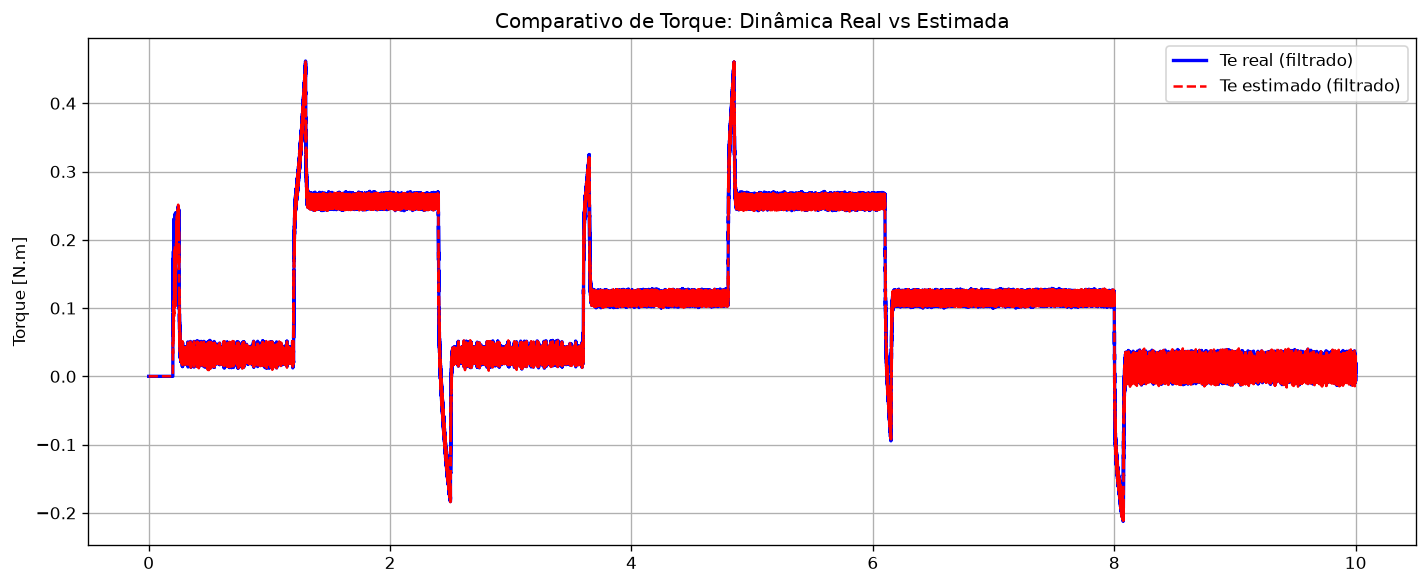
\includegraphics[width=0.8\linewidth,height=0.5\textheight,keepaspectratio]{figuras/torque_helice_17x10E.png}
  \fonte[Autor; APC Propellers (2026); Selig (2026)]
\end{frame}

\begin{frame}{Escolha do sensor de corrente}
  \centering
  \includegraphics[height=0.3\textheight]{Desenvolvimento/Captura de tela de 2026-05-16 16-12-58.png}\\[0.2em]
  {\small Primeira ideia: \textit{shunt} com amplificador isolado}\\[0.8em]
  \tikzfig{0.95}{0.36}{escolha_sensor}
  \fonte[Texas Instruments (2020); Ziegler et al.\ (2009)]
\end{frame}

\begin{frame}{Placas de aquisição}
  \begin{columns}[c]
    \begin{column}{0.36\textwidth}
      \centering
      \includegraphics[width=\linewidth]{Metodologia/placa aq1 SAME.png}\\[0.3em]
      {\small Projeto da AQ1}
    \end{column}
    \begin{column}{0.3\textwidth}
      \centering
      \includegraphics[width=\linewidth]{Resultados/pcb_feita_aq1.jpg}\\[0.3em]
      {\small AQ1 fabricada}
    \end{column}
    \begin{column}{0.3\textwidth}
      \centering
      \includegraphics[width=\linewidth]{Metodologia/gabinete.jpg}\\[0.3em]
      {\small Gabinete}
    \end{column}
  \end{columns}
  \fonte
\end{frame}

\begin{frame}{Sensor de corrente: caracterização}
  \begin{columns}[c]
    \begin{column}{0.4\textwidth}
      \centering
      \includegraphics[width=\linewidth]{Resultados/ensaio_sensor_corrente.jpg}
    \end{column}
    \begin{column}{0.6\textwidth}
      \centering
      \tikzfig{1}{0.68}{sensor_ss49e}
    \end{column}
  \end{columns}
  \fonte[Autor; Northrup (2018)]
\end{frame}

\begin{frame}{Lógica de aquisição}
  \centering
  \tikzfig{1}{0.75}{same_seq}
  \fonte[Autor; Zephyr Project (2026b)]
\end{frame}

\begin{frame}{Validação com \textit{breakpoints}}
  \ilustrativo
  \begin{columns}[c]
    \begin{column}{0.36\textwidth}
      \begin{itemize}
        \item Depuração direto na placa
        \item Cada etapa conferida em pausa
        \item Mesmo código do \textit{native\_sim}
      \end{itemize}
    \end{column}
    \begin{column}{0.64\textwidth}
      \centering
      \placeholder{8.5cm}{5.2cm}{Captura da sessão de depuração\\com \textit{breakpoints}}
      \fonte
    \end{column}
  \end{columns}
\end{frame}

\begin{frame}{Ensaio integrado}
  \ilustrativo
  \begin{columns}[c]
    \begin{column}{0.36\textwidth}
      \begin{itemize}
        \item SIBA e SAME sincronizadas
        \item Tração, torque e rotação no mesmo registro
        \item Exportação em CSV
      \end{itemize}
    \end{column}
    \begin{column}{0.64\textwidth}
      \centering
      \placeholder{8.5cm}{5.2cm}{Tração e torque estimado\\em função da rotação\\(ensaio integrado)}
      \fonte
    \end{column}
  \end{columns}
\end{frame}
